\documentclass[12pt]{article}
\usepackage{amsmath}
\usepackage{amssymb}

\title{The Discharge of a battery}
\author{Chris Walker}
\date{March 2,2020}

\usepackage{graphicx}
\usepackage{caption}
\usepackage{refstyle}

\begin{document}
\maketitle

\section{Introduction}
Batteries use up limited reagents in order to initiate a chemical reaction that produces electrons. These electrons provide the energy needed for the circuit to operate. Once a battery voltage is 4.8V the battery is considered “dead”.
The purpose of this experiment is to determine the life of a 9V battery.

\begin{figure}[h]
\begin{center}
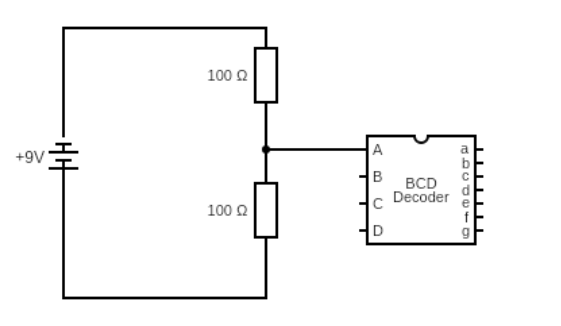
\includegraphics[width=0.8\textwidth]{Circuit_Design}
\caption{Circuit Diagram}
\label{fig:circuit}
\end{center}
\end{figure}

\section{Circuit Design}
The circuit that was used in this diagram was a circuit divider. As shown in \figref{circuit} a $9V$ battery was connected to an ADC 10 bit channel. The resistors that were used in the experiment each had a resistance of $100,\Omega$.These resistors were connected to a $5V$ and a $0V$ power rail in order to control the current of the battery. From there the first channel of the ADC chip was used to read the voltage, and current given by the battery.

\begin{figure}[h]
\begin{center}
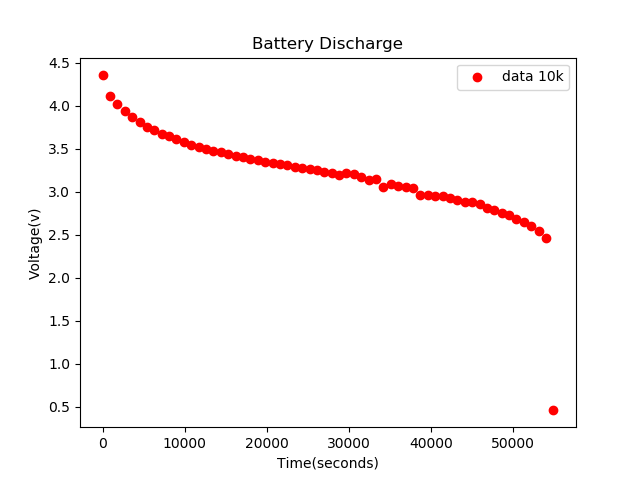
\includegraphics[width=0.8\textwidth]{VoltageDisch_all}
\caption{Continuous discharge of an Energizer 9V battery}
\label{fig:voltage}
\end{center}
\end{figure}

\begin{figure}[h]
\begin{center}
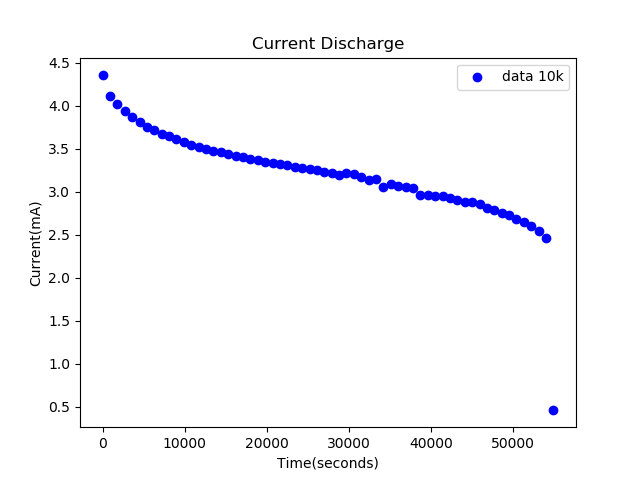
\includegraphics[width=0.8\textwidth]{CurrentDisch_all}
\caption{Charge of the Battery}
\label{fig:charge}
\end{center}
\end{figure}

\section{Result}
As illustrated in \figref{voltage}, the voltage of the  given battery dropped after thirteen hours of continuous drainage. A battery is considered“dead” when the voltage is equivalent to 4.8 volts. However in the experiment the voltage that was recorded is half of the voltage of the battery. This is due to Kirchhoff’s law. The circuit’s equation was given to be $\Delta,V_bat=,\Delta,V_1,+,\Delta,V_2$ and considering that $\Delta,V=R*I$, $\Delta,V_bat = R*I + R*I$.The resistance of the resistors was equal to $100\Omega$ and considering that they were in series $\Delta,V_bat=2,\Delta,V$ .Thus the voltage of the battery is equal to half of the voltage. In order to determine the charge of the battery an the integral $Q=,\int_{t_end}^{t_start}$. However, since this data was recorded over a span of seventeen hours it would be a rather difficult to find the integral. So in order to find the total charge the summation $Q=\sum_{i=1}^{n}{I_i,\Delta}$. The charge given off by the battery was determined to be 667.85 Columns.
\end{document}